\documentclass[12pt, titlepage]{article}
\usepackage{float}
\usepackage{changepage}
\usepackage{fancyhdr}
\usepackage{booktabs}
\usepackage{tabularx}
\usepackage{hyperref}
\usepackage{graphicx}
\usepackage{titling}
\usepackage[utf8]{inputenc}
\usepackage{graphicx}
\usepackage{gensymb}
\usepackage{siunitx}
\graphicspath{{./images/}}
\usepackage{array}
\graphicspath{ {figures/} }

\hypersetup{
    colorlinks,
    citecolor=black,
    filecolor=black,
    linkcolor=blue,
    urlcolor=blue
}
\usepackage[round]{natbib}
\begin{document}

\title{
    MobiCharged\\Hazard Analysis
    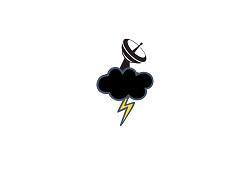
\includegraphics[width=9cm]{images/mobicharged.png} 
}
\author{Team Super Charged (No.33)
		\\ Nashit Mohammad - mohamn31
		\\ Eric Nguyen - nguyee13
		\\ Samuel De Haan - dehaas1
		\\ Eamon Earl - earle2
		\\ Mustafa Choueib - choueibm
}
    

\date{March 14, 2023, Rev. 1}


\maketitle

\pagenumbering{roman}
\tableofcontents
\listoffigures
\listoftables

\vspace{20pt}


\newpage

\pagenumbering{arabic}

\section{Revision History}
\begin{center}
\begin{table}[H]
\caption{\bf Revision History}
    \begin{tabular}{p{2cm}p{3cm}p{2cm}p{6cm}}
    \hline
    \bf Author & \bf Date & \bf Version & \bf Description\\
    \hline
    All & October 19, 2022 & Rev 0 & Created first draft of document\\
    \hline
    Nashit & March 18, 2023 & Rev 1 & Updated "Scope" to "Scope of Hazard Analysis"\\
    \hline
    Nashit & March 18, 2023 & Rev 1 & Updated "Definitions and Assumptions" to be Specific to the Hazard Analysis\\
    \hline 
    Nashit & March 18, 2023 & Rev 1 & Updated FMEA Table \& Functional Architecture\\
    \hline 
    \end{tabular}
\end{table}
\end{center}


\section{Introduction}

\subsection{Purpose}
The purpose of this Hazard Analysis document is to examine the MobiCharged project in its stage of development to outline all potential hazards. These hazards include, but are not limited to safety risks, areas of failure and security issues. Along with the highlighted areas of potential hazards, solutions to remove these issues (or mitigate these issues at best) will be outlined.

\subsection{Background}
Engineers are tasked with design in construction to exceed requirements without hindering safety. Safety is a topic that is never missed within the industry and is continuously being highlighted amongst designs; especially as Engineers are reminded of their moral obligations to society by their awarded rings upon graduation. 
\par
As a current process, the construction industry places sensors within concrete spaces to continuously test and/or monitor the integrity of buildings during as well as after construction. Ultimately however, these sensors run out of battery and are required to be re-charged.
\par
The industry still faces challenges when attempting to charge these sensors with the method of remote charging as the current products that satisfy remote charging abilities are yet to be optimized. There are a significant number of buildings being built in the Greater-Toronto-Area, which is emphasized considering that 70\% of cranes within Canada are in just the GTA alone. To place innovation in the sub-field of safety within the industry, it is indeed a requirement to modernize the ability of producing efficient remote charging systems by having the design process optimized to provide the most effective results.
\par
The system-solution for this will be the development of MobiCharged. This system is separated into two separate components - the software for users as well as the hardware / prototype. 
\par
The software component of MobiCharged is a machine-learned system that will react to the input of users (in which the input will be the desired outputs / application requirements for the remote charging device) and provide the necessary results (these variables depending on the user inputs can be antenna types, layouts, wavelengths, phases, etc.)  in order to satisfy the user’s inputs such that they may proceed with producing the devices in a way that it is optimized. This software can be operated in any environment the user chooses such that it can be used in any computing system with sufficient speed, memory \& the required processors. 
\par
The hardware component of MobiCharged is a prototype to be developed for the purpose of demonstration as well as development for the software. This physical component will allow the system to be rooted to the core optimization problem in the real world, as it applies to real products. The physical system will allow placing absolute constraints and limitations into the software for optimal outputs in the software. In addition, this physical system can be implemented for an actual use-case in the field for demonstrations. The environments in which these physical systems operate are typically from roof-tops and/or high-altitude locations with spacial capabilities to place arrays of these systems. These systems react to user inputted (remotely) data such as the location of the device required to be charged, so that it may orient itself in a manner optimal for that application. 

\subsection{Scope of Hazard Analysis}
The objective of this hazard analysis is to identify any and ideally all potential hazards/risks project MobiCharged may encounter. Moreover, the goal is to evaluate the likelihood and severity of these risks while generating solutions to remove and/or mitigate them.
\par
The scope of the hazard analysis will be limited to the software system as well as the hardware system. The software system will be analyzed for anything that can create errors and/or issues for the users which include but are not limited to incorrect outputs, crashing of the software and security issues. The hardware system will be analyzed for anything that can bring harm to the user which includes voltage/current spikes, malfunction of hardware system and areas of physical danger. The project being analyzed will be analyzed for when it is in operation but also for the cases when it is not in operation. 

\subsection{Definitions \& Assumptions}

\subsubsection{Definitions}
\begin{table}[H]
\caption{\bf Naming Conventions and Terminology}
\begin{tabular}{ |p{6cm}|p{8cm}|  } 
 \hline
\bf Word & \bf Definition/Context\\
 \hline
 System Hazard & A hazard associated with the system which typically exists regardless of the status of operation.\\
 \hline
 Accident & An unintended event  which generally leads to a form of loss.\\
 \hline
 Risk & A probability of exposure to danger.\\
 \hline
 Phase-Shift System & A system designed to alter the waves distributed such that it moves the phase of a wave.\\
 \hline
 Antenna Array & A system of antenna designed to distribute waves in an organized layout.\\
 \hline
 ASCII Values & A standard data-encoding format for electronic communication between computers.\\
 \hline
 Output Limitation Timers & A software algorithm module designed to measure the time it takes for a process to complete and cancel the process if the time elapsed exceeds a programmed amount.\\
 \hline
 FR - Functional Requirement & Requirements that describe what the product is supposed to do\\
 \hline
NFR - Non-functional Requirement & Requirements that describe qualities that product will have\\
 \hline
General Contractor & Third party companies that acquire services by Mobilite-Power\\
  \hline
ECA & The Electrical Construction Association\\
\hline
Data Smoothing & The process of using old data as well as "future" data in order to predict designs.\\
\hline
ML & "Machine Learning" algorithm.\\
\hline
\end{tabular}
\end{table}

\subsubsection{Assumptions}
\begin{itemize}
    \item There is an assumption that the developers will eventually have access to enough processing power to conduct large quantities of simulations.
    \item A large underlying assumption regarding the software system is that the user does not intentionally attempt to enter inputs incorrectly, as well as provide positive feedback to the system when it is not correct.
    \item The user will be ages 14 and up for hardware system. Ages 16 and up for software system.
    \item The user has a fundamental background in hardware operation safety.

\end{itemize}


\section{Component Overview}

\subsection{Software System}
\subsubsection{Front End User Display}
The Front End User Display component is the component in which the user is able to view. This area is where the user navigates through the software, log-in their accounts, enters inputs, requests data and/or verification, and receives outputs.

\subsubsection{Back-End Calculations}
The Back-End Calculations component of the software system is for the computerized calculations to occur based on the user’s inputs. Note that this does not refer to simulations; this component is merely where the user’s inputs are calculated to higher level variables such that the software may then be used to process to create outputs. 

\subsubsection{Machine-Learning Algorithm}
The Machine-Learning component of this software system is where the system receives feedback either from the outputs themselves, or from the user in regards to desirable solutions. The more positive feedback it receives, the more of these inputs the system will retain. Similarly, the more negative feedback the system receives, the less of those specific inputs it will retain. As the system continues to learn, the concept of the system providing suggestions, limitations and of course the optimal solutions will become present. 

\subsubsection{Data Exporting}
The Data Exporting component of the software system is the area of the software system where it exports the results. This not only refers to merely outputting the data to the front-end display component, but also refers to exporting into desirable file systems to be stored as well as encryption processes during transfer. 

\subsubsection{Server}
The Server component will be used to maximize the training available to the machine learner, by having the simulations run on local machines, and passing the data via the online connections to an isolated machine and database, which will encapsulate the Machine-Learning Algorithm component. This will be in a future iteration of the design.

\subsubsection{Simulation Integration Software}
This component encompasses the pre-existing Matlab simulations with which we will integrate our machine learning algorithm, and the software required to integrate them. It will likely involve a database system as well as kernel modules for real-time polling of said database(s), with a dynamic scheduler. 

\subsection{Hardware Systems}
\subsubsection{Power Supply System}
The purpose of the power supply system component is to provide usable power to subsequent systems. 

\subsubsection{Phase-Shift System}
This component will work to provide the phase shift required for the antenna array system to properly create wave required interference. The purpose of this is to facilitate constructive interference at the desired location for charging. 

\subsubsection{Antenna-Array System}
This component will contain multiple small arrays and will work in conjunction with the Power Supply system and Phase-Shift System.

\subsubsection{System Enclosure}
This component is present to enclose the system. Typically, the material of this enclosure is a form of wave-reflective metal. The purpose of the enclosure is such that the waves create a destructive interference in the direction that it is not desired to go towards, and creates an amplified constructive interference in the direction that it is desired in. 

\subsubsection{Hardware Display System}
This component is for the user to understand when the device is operational, functional, etc. The current display system is under development, however, the use of LEDs will most likely be implemented. 

\subsubsection{Circuits \& Logic}
This will consist of any circuitry required for proper control and use of the overall system. 

\section{Failure Modes \& Effects Analysis Table}
Below is a failure modes and effects analysis (FMEA) for MobiCharged system.
\newpage
\fancyhf{}
\fancyhead[C]{\thepage}
\renewcommand{\headrulewidth}{0pt}
\pagestyle{fancy}
\begin{center}
\begin{adjustwidth}{-3.5cm}{}
\begin{tabular}{|p{1.5cm}|p{1.4cm}|p{1.5cm}|p{2cm}|p{3.5cm}|p{2cm}|p{1.4cm}|p{4.3cm}|}
\hline
Design Component & Ref.\# & Failure Modes & Causes of Failure & Effects of Failure & Detection & Controls & Recommended Action\\
\hline
Front End User Display & 4.1.1.0 \par(NFR11) & Incorrect Outputs & -Incorrect inputs from user \par -Incorrect input type \par -Unintended indexing in Database \par -Race Conditions & Users carry incorrect outputs that are later used to produce the remote charging devices. This results in a device produced that is not actually the one optimized for certain application & -Software can detect incorrect input types based on ASCII values \par -Other forms are not detectable & N/A & -Display confirmation screen containing inputs provided by the user \par -Display/Export the data of outputs along with the user's inputs at all times \par -Create an "Incorrect Input" pop-up display when the user enters an incorrect input type \par -Display examples of inputs for user \par -Display input limitations \par -Display a "Calculation Failed" screen if calculation fails (and have program execute fail-safe) \par -Ensure Race Conditions \& concurrency errors do not occur by correctly writing program to avoid it (eg: using semaphores) \par\\

 & 4.1.1.1 \par(NFR13) & Frozen Screen and/or Crash & -User inputs values exceeding calculation capabilities (eg;dividing by 0) \par -Removal of power to software system during process \par -Deadlock & -Reboot necessary \par -Loss of data & -Interrupted process by loss of data (only detected once in operation again) & N/A & -Avoid incorrect programming that may cause deadlocks and ensure robustness in code \par -Limit users from inputting incorrect data \par -Provide users examples of acceptable data types \par -Produce an emergency module that informs user of the loss of data after the crash, while advising them to report the issue to the manufacturer if repeated continuously\\
 \hline
\end{tabular}
\end{adjustwidth}
\end{center}


\begin{center}
\begin{adjustwidth}{-3.5cm}{}
\begin{tabular}{|p{1.5cm}|p{1.4cm}|p{1.8cm}|p{2cm}|p{3.5cm}|p{1.7cm}|p{1.5cm}|p{4.2cm}|}
\hline
Design Component & Ref.\# & Failure Modes & Causes of Failure & Effects of Failure & Detection & Controls & Recommended Action\\
\hline
Front End User Display & 4.1.1.2 \par(NFR4)& Incorrect Login Information & User forgets password and/or username & Loss of previous data history for user & N/A & N/A & -Generate security questions during account creation, thus, if user forgets password they can reset it using security questions \par -Make software tied to online servers, allowing users to get a reset link their email address\\
 \hline
 Backend Calculations & 4.1.2.0 \par(SR4)& Failed Calculations (undefined answers) & -User enters values that lead to undefined answers \par -User enters incorrect data types \par -User enters extreme data values & -Crash of calculations and no outputs \par -Potentially outputting incorrect data without warning, which could then be used to produce remote charging devices & N/A & N/A & -Limit the data types users can input based on ASCII values \par -Ensure correct and sufficient testing is implemented during development\\
 \hline
 Machine Learning Algorithm & 4.1.3.0  \par (NFR5)& Infinite loop & -Incorrect programming \par -Negligence of exiting loops & -Software crash \par -Computer crash \par -Reboot system \par -Loss of data & -Computer built-in exiting programs \par -Output limitation timers & N/A & -Ensure correct programming to avoid infinite loops \par -Enter states of polling to ensure processing does not exceed time limits \par -Create failure states within code\\
 & 4.1.3.1 \par(NFR13) & Incorrect Data-Smoothing & -Ineffective algorithms implemented \par -Limit of data present & -Incorrect data output leading to non-optimized solutions and devices \par -Catastrophic errors may occur if positive feedback is provided to incorrect output & N/A & N/A & -Produce extensive research to implement the most effective data-smoothing algorithm \par -Increase data set overtime \\
 \hline
\end{tabular}
\end{adjustwidth}
\end{center}



\begin{center}
\begin{adjustwidth}{-3.5cm}{}
\begin{tabular}{|p{1.6cm}|p{1cm}|p{1.8cm}|p{2.4cm}|p{3cm}|p{1.7cm}|p{1.5cm}|p{4.5cm}|}
\hline
Design Component & Ref.\# & Failure Modes & Causes of Failure & Effects of Failure & Detection & Controls & Recommended Action\\
\hline
Machine Learning Algorithm & 4.1.3.2 \par (SR2) & Positive feedback applied to incorrect results (mislabelled data) & -Incorrect algorithms implemented \par Feedback entered incorrectly, repeatedly & -Catastrophic as incorrect outputs will be produced every time \par -Incorrect data will be implemented when producing remote charging devices \par -System failure as a whole & Comparison through data & N/A & -Apply verification checks periodically to machine-learned algorithm to ensure it matches up correctly to existing solutions and data \par -Disallow users from directly inputting labelled data (can only be passed as the output to a simulation)\\
\hline
Data-Exporting & 4.1.4.0 \par(SR3)& Unable to export & -Export file type not supported \par -Exporting process stopped due to higher priority preemption or power loss during process & -Exporting failed, data is not exported to user \par -Data is not saved & -Software check \par -Computer built in exit programs & N/A & -Provide user the requirements of installing the software to ensure the necessary support is present \par -Deny the installation of the software system if necessary support is not present \par -Create the programs modular and preemptable such that the process can continue after halt\\
& 4.1.4.1 \par (SR4)& Incorrect data outputted & -Race conditions \par -Incorrect indexing through data &  Incorrect solution provided &Visual check between correct data displayed to user and exported data & N/A & -Thorough programming to avoid race conditions \par -Apply verifications to ensure indexing is correct\\
&4.1.4.2 \par(NFR17)& Vulnerable data & -Data leaks & Possibly critical client data available to malicious parties & Ethical hacking attempts to assess vulnerabilities & N/A & Encrypt outbound data on local machines before transmitting via the server (SR3)\\
\hline 
\end{tabular}
\end{adjustwidth}
\end{center}

\begin{center}
\begin{adjustwidth}{-3.5cm}{}
\begin{tabular}{|p{1.6cm}|p{1cm}|p{1.8cm}|p{2.4cm}|p{3cm}|p{1.7cm}|p{1.5cm}|p{4.5cm}|}
\hline
Design Component & Ref.\# & Failure Modes & Causes of Failure & Effects of Failure & Detection & Controls & Recommended Action\\
\hline
Server & 4.1.5.0 \par (SR5)& Server inaccessible & -Server at capacity \par -server hardware malfunction / internet access restricted & -Inability to serve users \par -Loss of data & An inevitable hazard, must use recommended actions as fail-safes & N/A &-Timeout for idle clients on the server \par -Local backups of un-transmitted data\\
\hline 
Simulation Integration Software & 4.1.6.0 \par (SR6)& Inaccurate results & -computational error & Our Machine-Learning Algorithm may only achieve a certain percent accuracy at best, even with infinite labelled input data & -Development of hardware, and comparison between Matlab simulation output and real-world testing & N/A & If error found to be large, alterations of the simulations would be in order to purify the data fed to our learner\\
&4.1.6.1 \par(SR1)& Data overflow & -Simulations produce outputs faster than can be processed by the ML algorithm, or considerably faster than the server polling speed & Simulation data is lost as the queue is at capacity & Have a flag for when overflow occurs & N/A & -Dynamic polling speeds, for increase in clients using the server in the future \par -Third party database monitoring software, for if simulation speeds greatly increase down the line\\
\hline
\end{tabular}
\end{adjustwidth}
\end{center}




\begin{center}
\begin{adjustwidth}{-3.5cm}{}
\begin{tabular}{|p{1.6cm}|p{1.2cm}|p{1.6cm}|p{2.4cm}|p{2cm}|p{2.2cm}|p{2cm}|p{4.5cm}|}
\hline
Design Component & Ref.\# & Failure Modes & Causes of Failure & Effects of Failure & Detection & Controls & Recommended Action\\
\hline
Power Supply System & 4.2.1.0 (NFR12)& No power supplied to subsequent systems & -Fault in power supply \par -Fault in power supply cables to downstream systems & -System crash \par -Loss of data & Current measurements taken at antenna-array system & N/A & -Disconnect power supply system from remaining systems \par -Conduct testing of power supply components to determine mode of failure \par\\

& 4.2.1.1\par (NFR12) & Voltage swell & Large change in loads seen by power system & System short circuited & Voltage measurements taken at antenna-array system & Protection devices (fuses) downstream from power supply & Conduct testing of power supply components to determine mode of failure\\
\hline
Phase-Shift System & 4.2.2.0 \par (NFR6) & Phase shifter component failure & Component break down & - System failure \par - Incorrect phase applied to system and unintended waves will be created \par - Device intended to be charged may not be charged & Measurement of induced radio waves & N/A & Testing of units prior to assembly\\
\hline
Antenna Array System & 4.2.3.0 \par (NFR6) & Antenna Array Component failure & -Component break down \par -Over current supplied & - System Failure \par - Waves will not be distributed \par - Devices will not be charged & Measurement of induced radio waves & Protection devices (fuses) to limit current to antenna within operating range & -Testing of units prior to assembly \par -Monitor power supplied to units\\
\hline
\end{tabular}
\end{adjustwidth}
\end{center}

\begin{center}
\begin{adjustwidth}{-3.5cm}{}
\begin{tabular}{|p{1.6cm}|p{1.2cm}|p{1.6cm}|p{2.0cm}|p{3.7cm}|p{2cm}|p{2cm}|p{3.5cm}|}
\hline
Design Component & Ref.\# & Failure Modes & Causes of Failure & Effects of Failure & Detection & Controls & Recommended Action\\
\hline
System Enclosure & 4.2.4.0 \par (NFR12) & Enclosure "leak" & Gap in wave reflective enclosure system & - Waves will leak through the gap and constructive interference will occur in unintended directions \par - The intended directions for the waves to be distributed will be minimized; device may not be charged due to length of waves not sent  & -Measurement of induced radio waves \par -Visual inspection & N/A & -Inspection prior to use \par -Remove sensitive equipment from affected area\\
\hline
Hardware Display System & 4.2.5.0 \par (NFR12) & False indication & Display stuck in "on" or "off" state & - Confusion amongst user \par - Incorrect usage may occur by user & Verification downstream to determine state of device & Wire indication in line with power supply to device & Disconnect the device from the power supply system until failure mode has been determined\\
\hline
\end{tabular}
\end{adjustwidth}
\end{center}

\fancyhf{}
\fancyhead[C]{\thepage}
\renewcommand{\headrulewidth}{0pt}
\pagestyle{plain}


\section{Functional Architecture}
As many constraints require feasible prototypes, the requirements are subject to change accordingly.
\subsection{Functional Requirements}
\subsubsection{Software System Functional Requirements}
\textbf{SR1.} ML Model must optimize inputs faster than the existing process.\\
\textbf{SR2.} ML Model must be able to develop "new" simulations based on previous optimal models.\\
\textbf{SR3.} ML Model must be able to encrypt optimized data before exporting for the purpose of security and privacy.\\
\textbf{SR4.} The software system must determine and output the optimized and correct solution.\\
\textbf{SR5.} ML Model must be able to process incoming simulation data from multiple source devices.\\
\textbf{SR6.} ML Model must be able to interpret data exported directly from Matlab simulations.

\color{black}

\subsubsection{Hardware System Functional Requirements}
\textbf{HR1.} The system must be able to simulate a remote charging device by levitating a particle in an air medium within the hardware capsule for at least 5 minutes.\\
\textbf{HR2.} The system must be able to levitate the particles for simulation purposes within 15 seconds.\\

\subsection{Non-functional Requirements}
\subsubsection{Look and Feel Requirements}
\textbf{NFR1.} The hardware system will be packaged neatly such that all wiring is hidden and not exposed to the users.\\
\textbf{NFR2.} The software system will be produced with front end design colors such that strains to the eye are minimized.
\subsubsection{Appearance Requirements}
\textbf{NFR3.} The system will consist of a simple user interface by minimizing unnecessary and complex functionalities.

\subsubsection{Access Requirements}
\textbf{NFR4.} Authorized users will have access to the system while unauthorized users will not.

\subsubsection{Integrity Requirements}
\textbf{NFR5.} The system must be able to store its current state locally in the event of a failure.\\
\textbf{NFR6.} The individual components of the physical system must be inspected and tested.

\subsubsection{Style Requirements}
N/A
\subsubsection{Usability and Humanity Requirements}
N/A
\subsubsection{Ease of use Requirements}
\textbf{NFR7.} The system shall be simple to install within 10 steps and within one hour.

\subsubsection{Learning Requirements}
\textbf{NFR8.} The system shall be understandable within an hour of use.

\subsubsection{Understandability and Politeness Requirements}
N/A

\subsubsection{Speed and Latency Requirements}
\textbf{NFR9.} The system must compute optimal configuration within 6 hours.

\subsubsection{Safety Critical Requirements}
\textbf{NFR10.} The hardware system must have a fail safe option such that at the system shuts off at the event of failure to reduce potential harm.

\subsubsection{Precision of Accuracy Requirements}
\textbf{NFR11.} The system must have a relative accuracy of 5\% compared to current Matlab simulation.

\subsubsection{Reliability and Availability Requirements}
\textbf{NFR12.} The system must be available at all times.\\

\subsubsection{Robustness of Fault Tolerance Requirements}
\textbf{NFR13.} The system must be able to discard any corrupted data without adding it to the database.\\

\subsubsection{Capacity Requirements}
N/A
\subsubsection{Physical Environment}
\textbf{NFR14.} The hardware system must be able to withstand an input of an upper limit of 15 volts\\

\subsubsection{Release Requirements}
N/A
\subsubsection{Maintenance Requirements}
N/A

\subsubsection{Adaptability Requirements}
\textbf{NFR15.} The system must be functional on Windows and macOS.

\subsubsection{Security Requirements}
NFR17 - Client data must be protected.

\subsubsection{Access Requirements}
N/A

\subsubsection{Privacy Requirements}
\textbf{NFR16.} The system must encrypt all exported data.


\subsubsection{Legal Requirements}
N/A

\subsubsection{Health and Safety Requirements}
N/A

\section{Conclusion}
Designing a software system is an intricate process, one that requires an inhuman-like insight into the very minute details of various sub-systems, independently nuanced and dependently coupled. For these reasons, they often contain far more mistakes and vulnerabilities than their proud creators suspect or even care to believe. This fact underlines the importance of acknowledging our faults and the likely faults of our current designs, which in turn allows us to not only protect against them but also further iterate on our pre-existing plans for development. By highlighting these hazards, we have been forced to further understand and define the constraints that are laid around our problem space, and how we might work to achieve all of them and the safest system possible. It is also important to notice the cyclical nature of data flow in our system, which can be seen in the various diagrams showing our system context in SRS Rev 0; thus our software system is especially vulnerable to the propagation of errors, and to the injection of poor data. In looking at the vulnerabilities we have been forced to understand the internal communications of all of our main components - the nature of their coupling as well as their own modular behaviour. The state of our problem definition, goals, and development plan are all better for it.

\section*{References}
We will be referring to documentations provided by Mobilite-Power, however, as of now there are no references to mention.




\end{document}

